\documentclass[fleqn]{article}
\usepackage[left=1in, right=1in, top=1in, bottom=1in]{geometry}
\usepackage{mathexam}
\usepackage{amsmath}
\usepackage{graphicx} 
\usepackage{latexsym}
\usepackage{polski}
\usepackage[utf8]{inputenc}
\usepackage{listings}
\usepackage{color}
\definecolor{codegreen}{rgb}{0,0.6,0}
\definecolor{codegray}{rgb}{0.5,0.5,0.5}
\definecolor{codepurple}{rgb}{0.58,0,0.82}
\definecolor{backcolour}{rgb}{0.95,0.95,0.92}
\lstdefinestyle{mystyle}{
    backgroundcolor=\color{backcolour},   
    commentstyle=\color{codegreen},
    keywordstyle=\color{magenta},
    numberstyle=\tiny\color{codegray},
    stringstyle=\color{codepurple},
    basicstyle=\footnotesize,
    breakatwhitespace=false,         
    breaklines=true,                 
    captionpos=b,                    
    keepspaces=true,                 
    numbers=left,                    
    numbersep=5pt,                  
    showspaces=false,                
    showstringspaces=false,
    showtabs=false,                  
    tabsize=2
}
 
\lstset{style=mystyle}

\ExamClass{MDM}
\ExamName{Lista I}
\ExamHead{\today}
\author{Michał Bronikowski}
\let\ds\displaystyle

\begin{document}
\ExamInstrBox{
\begin{center}
Michał Bronikowski \\
Deklaruję zadania numer: 2,7,8,10,13,14
\end{center}
}
\hfill
\\
\\
\\
\\
\\
\\
\[\huge \bf Zadanie \ 2\] 
Uporządkuj od najwolniej do najszybciej rosnącej funkcje (logarytmy mają podstawę 2): \\ \\
\begin{center} $
\log n ,
(\log n) ^{n} ,
n^{\log n} ,
\log (n^{n}) ,
3 ^ {\log n} ,
n ,
n^{2} ,
2^{\sqrt{n}} ,
1.01^{n} ,
0.99^{n} ,
(1 +\frac{1}{n} ) 
$
\end{center}
Rozwiązanie: \\
Na początku przekształciłem sobie podane funkcje do postaci:(Z zachowaniem kolejności z treśći) \\
\begin{center}$
\log n \newline \newline
(\log n) ^{n} = 2^{\log n ^{\log n}} = 2^{\log n \times {\log n}}=2^{\log^{2} n} \newline \newline
n^{\log n} = (\log n) ^{n} = 2^{\log \log n^{n}} = 2^{\log \log n \times n}\newline \newline
\log (n^{n}) = n \times \log n \newline \newline
3 ^ {\log n} = 2 ^{\log 3 ^{\ log n}} = 2^{\log n \times \log 3} = n ^{\log 3} \newline \newline
n \newline \newline
n^{2} = 2^{\log n \times 2}\newline \newline
2^{\sqrt{n}} \newline \newline
1.01^{n} = 2^{\log 1.01^{n}} = 2^{n \times \log 1.01} \newline \newline
0.99^{n} // Funkcja \ jest \ malejąca \newline \newline
(1 +\frac{1}{n} ) = e\newline \newline
$
\end{center}
Funkcje ułożone w kolejności od najwolniej rtosnącej do najszybciej to: \newline \newline
\begin{center}
$
0.99^{n} \prec (1 +\frac{1}{n} ) \prec \log n  \prec n \prec \log (n^{n})  \prec 3 ^ {\log n} \prec n^{2} \prec n^{\log n} \prec 2^{\sqrt{n}} 
\prec 1.01^{n} \prec  (\log n) ^{n} 
$
\end{center}
Uzasadnienie:\\
 najwolniej rośnie $ 0.99^{n} $, ponieważ jest to funkcja malejąca -- zbieżna do zera. Druga w kolejności jest funkcja $(1 +\frac{1}{n} )$, ponieważ zbiega do $e \approx 2.71 $. Następna jest funkcja $\log n $, która rośnie szybciej od poprzednich, ale wolniej od $n$ -- które łatwo porównać do pozostałych funkcji. Następna w koleności funkcja to właśnie $n$, którą w prosty sposób można porównać z pozostałymi przedstawionymi w postaci  $2^{x}$ ,$n ^{\log 3} $lub $n \times \log n$. Następna funkcja to $\log (n^{n}) $, którą porównuję z pozostałymi funkcjami w postaci   $2^{x}$ ,$n ^{\log 3} $i stwierdzam, że rośnie od nich ,,wolniej". Następnie z pozostałych funkcji zostaje jedna , która nie jest postaci $2^{x}$ czyli : $3 ^ {\log n}$. Następnie porównuję wykłądniki w pozostałych funkcjach postaci $2^{x}$ i ustawiam je w kolejności od najwolniej rosnącego  do najszybciej tj.: \\ \\ \\
 $
 2^{\log n \times 2} \newline\newline
 2^{\log \log n \times n} \newline\newline
 2^{\sqrt{n}} \newline\newline
 2^{n \times \log 1.01} \newline\newline
 2^{\log^{2} n} \newline\newline
 $
 \begin{flushright}
 $\Box$
 \end{flushright}
 \[\huge \bf Zadanie \ 7\] 
 Rozważmy algorytm sortujący n liczb w następujący sposób. Wybierz najmniejszą, postaw na pierwszym miejscu, wybierz następną najmniejszą i postaw na drugim miejscu, następną postaw na trzecim miejscu itd. aż do wyczerpania liczb. Określ złożoność czasową powyższej procedury.\\ \\ \\
 Na początku mamy $n$ liczb wybieramy pierwszą z brzegu i porównujemy ją z $(n-1)$ liczbami, aby wybrać najmniejszą. Następnie mamy $(n-1$ liczb i porównujemy je z $(n-2)$ liczbami itd. aż zostanie mi ostani wyraz, który porównam z $0$ liczb. Suma tych wszystkich wyrazów jest postaci: \\ \\
 $
 \sum_{i=1}^{n-1}i \newline \newline
 $
 Jest to szereg arytmetyczny, którego suma jest równa: \\ \\
 $
 S_{n} =\frac{a_{1} +a_{n}}{2} \times n = \frac{1 + n -1}{2} \times n = \frac{n}{2} \times n \newline \newline   
 $
 Więc złożoność czasowa tej procedury to: 
 $
 \mathcal{O}(n^2) \newline \newline
 $
 \newpage
 \[\huge \bf Zadanie \ 8\] 
 Oceń złożoność czasową pisemnego dodawania i mnożenia. \\ \\
 \begin{itemize}
 \item[•] Dodawanie \\ \\
 Dodając pisemnie do siebie dwie liczby o $n$ cyfrach wykonujemy maksymalnie $n$ dodawań plus $n-1$ przeniesień.\\
 Złożoność :  
 $
 \mathcal{O}(n) \newline \newline
 $
 \item[•] Mnożenie \\ \\
 Mam $n\ \times $  (n mnożeń + (n - 1) przeniesień) + n dodawań liczb dlugości (2n - 1) cyfr + maksymalnie (2n -2) przeniesienia w dodawaniu.
 \\ \\Złożoność:
  $
 \mathcal{O}(n^{2}) \newline \newline
 $
 \end{itemize}
 \[\huge \bf Zadanie \ 10\] 
Używając całkowania (oszacuj podobnie jak na wykładzie) sumę: \\ \\
$
\sum_{k=1}^n = \frac{1}{k} \newline \newline
$ 
Na początku tak jak na wykładzioe narysowałem sobiue wykres pomocniczy: \\ \\
\begin{center}
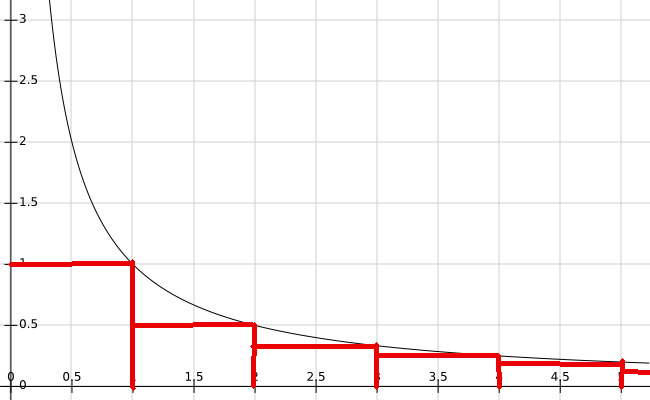
\includegraphics[width=\textwidth]{zad10-wykres} 
\caption{Rysunek pomocniczy -- funkcaj $\frac{1}{x}$ i prostokąty o szerokości $1$
\end{center}
\\ \\Pole pod wykresem jest równe: \\ \\
\[\int_{1}^{n}\frac{1}{x} = \ln n - \ln 0 = \ln n\]
Wszystkie ,,błędy" obliczeniowe ,,mieszczą" się w pierwszym prostokącie, więc należy odjąć $\mathcal{O}(1)$ \\ \\Ostateczny wynik jest postaci:
\textbf{$\ \ln n - \mathcal{O}(1) \newline \newline$}
  \begin{flushright}
 $\Box$
 \end{flushright}
\[\huge \bf Zadanie \ 13\]
 Wykaż, że ilość liczb całkowitych w następujących przedziałąch są odpowiednio równe $(a<b)$: \\
 \begin{itemize}
 \item[a)] $\langle a,b) \ -- \ \lfloor b\rfloor - \lceil a\rceil + 1 $\\
  Najmniejsza liczba w tym przedziale to: $\ \lceil a\rceil $\\
  Największa liczba w tym przedziale to: $\ \lfloor b \rfloor $\\
  Ilość liczb w tym przedziale jest więc równa:$\ \lfloor b \rfloor - \lceil a\rceil  + 1 $ \\
  
  \item[b)] $\langle a,b) \ -- \ \lfloor b \rfloor - \lceil a \rceil$\\
  Najmniejsza liczba w tym przedziale to: $\ \lceil a\rceil $\\
  Największa liczba w tym przedziale to: \\ \\
  Dla $b\in\mathbb{Z}$ $\ \lfloor b \rfloor -1 $\\
  Dla $b\notin\mathbb{Z}$ $\ \lfloor b \rfloor $\\
  Ilość liczb w tym przedziale jest więc równa: \\ \\
  Dla $b\in\mathbb{Z}$ $\ \lfloor b\rfloor - 1 - \lceil a\rceil +1 \ // i \ \ \lfloor b\rfloor =\lceil b\rceil  \\Podstawiając:\lceil b\rceil - \lceil a\rceil$\\ \\
  Dla $b\notin\mathbb{Z}$ $\lfloor b\rfloor - \lceil a\rceil +1 \ // i \ \ \lfloor b\rfloor =\lceil b\rceil -1 \\Podstawiając:\lceil b\rceil - \lceil a\rceil $\\
  
  \item[c)] $(a,b\rangle \ -- \ \lfloor b\rfloor - \lfloor a \rfloor$\\
  Najmniejsza liczba w tym przedziale to:\\ \\
  Dla $a\in\mathbb{Z}$ $\ \lceil a\rceil + 1 $\\
  Dla $a\notin\mathbb{Z}$ $\ \lfloor b \rfloor $\\
  Największa liczba w tym przedziale to: $\ \lceil a\rceil$\\
  Ilość liczb w tym przedziale jest więc równa:\\ \\
  Dla $a\in\mathbb{Z}$ $\ \lfloor b\rfloor - \lceil a\rceil-1 +1 \ // i \ \ \lfloor a\rfloor =\lceil a\rceil  \\Podstawiając:\lfloor b\rfloor - \lfloor a\rfloor $\\ \\
  Dla $a\notin\mathbb{Z}$ $\ \lfloor b\rfloor - \lceil a\rceil+1 \ // i \ \ \lceil a\rceil  =\lfloor a\rfloor-1  \\Podstawiając:\lfloor b\rfloor - \lfloor a\rfloor$\\

  \item[d)]$(a,b) \ -- \ \lceil b \rceil -\lfloor a\rfloor - 1$ \\
  \begin{enumerate}
	\item Dla $a\in\mathbb{Z} \ i \ b\notin\mathbb{Z} $\\
		 Najmniejsza liczba w tym przedziale to: $\ \lceil a\rceil +1 $\\
         Największa liczba w tym przedziale to: $\ \lfloor b \rfloor $\\
         Ilość liczb w tym przedziale jest więc równa:$\ \lfloor b \rfloor - \lceil a\rceil -1+1=\lfloor b\rfloor-\lceil a\rceil = \lceil b\rceil -\lfloor a\rfloor -1$ \\
	\item Dla $a\notin\mathbb{Z} \ i \ b\in\mathbb{Z} $\\
		 Najmniejsza liczba w tym przedziale to: $\ \lceil a\rceil $\\
         Największa liczba w tym przedziale to: $\ \lfloor b \rfloor -1$\\
         Ilość liczb w tym przedziale jest więc równa:$\lfloor b \rfloor - 1 - \lceil a\rceil +1=\lfloor b\rfloor-\lceil a\rceil = \lceil b\rceil -\lfloor a\rfloor -1$ \\
     \item Dla $a\notin\mathbb{Z} \ i \ b\notin\mathbb{Z} $\\
		 Najmniejsza liczba w tym przedziale to: $\ \lceil a\rceil $\\
         Największa liczba w tym przedziale to: $\ \lfloor b \rfloor $\\
         Ilość liczb w tym przedziale jest więc równa:$\lfloor b \rfloor  - \lceil a\rceil +1=\lceil b\rceil-1-\lfloor a\rfloor-1+1 = \lceil b\rceil -\lfloor a\rfloor -1$ \\
     \item Dla $a\in\mathbb{Z} \ i \ b\in\mathbb{Z} $\\
		 Najmniejsza liczba w tym przedziale to: $\ \lceil a\rceil +1 $\\
         Największa liczba w tym przedziale to: $ \lfloor b \efloor -1$\\
         Ilość liczb w tym przedziale jest więc równa:$\lfloor b \rfloor  -1- \lceil a\rceil-1 +1 = \lceil b\rceil -\lfloor a\rfloor -1$\\
\end{enumerate}
  \end{itemize}  
\[\huge \bf Zadanie \ 14\] 
Pokaż, że dla dowolnego $x\geq0$: \\ \\
$
\lfloor\sqrt{x}\rfloor = \lfloor\sqrt{\lfloor x \rfloor} \rfloor \newline \newline
$
Rozwiązanie: \\ \\
FAKT: \\ \\
$
x \leq \lfloor x\rfloor \Rightarrow \sqrt{x} \geq \sqrt{\lfloor x \rfloor} \Rightarrow \lfloor \sqrt{x} \rfloor \geq\lfloor \sqrt{\lfloor x \rfloor} \rfloor \newline \newline 
$
$
\exists_{a\in\mathbb{N}}\ \ \ a\leq\lfloor x \rfloor \leq x \leq a + 1 \newline \newline
$
Ponadto da się znaleźć takie c, że: \\ \\
$
\exists_{a,b\in\mathbb{N}}\ \ \ c^{2} \leq a\leq\lfloor x \rfloor \leq x \leq a + 1 \leq (c+1)^2 \newline \newline
$
\begin{itemize}
\item[•] Dla $x = 0$ ta nierówność jest oczywista dla $a,b = 0$. Zarówno dla $x=0$ nierówność
$\lfloor\sqrt{x}\rfloor = \lfloor\sqrt{\lfloor x \rfloor} \rfloor $ jest prawdziwa.
\item[•] Dla $x>0$. Możemy nierównośc przekształcić w następujący sposób : \\ \\
\begin{center}
$ c^{2} \leq \lfloor x \rfloor \leq x \leq (c+1)^2 /\sqrt{}\newline \newline$
$ c \leq \lfloor \sqrt{x} \rfloor \leq \sqrt{x} \leq (c+1) \newline \newline$
\end{center}
Wiem, że $c$ jest liczbą naturalną więc jeżeli w nierówności występuje podłoga, która sprowadza $\sqrt{x}$ do części całkowitej i $\lfloor \sqrt{x} \rfloor \leq \sqrt{x}$ jest ograniczone przez dwie kolejne liczby naturalne to:$\lfloor \sqrt{x} \rfloor$ jest równy $ \sqrt{x} $
 \begin{flushright}
 $\Box$
 \end{flushright}


\end{itemize}
\end{document}

